\documentclass[border=3pt]{standalone}
% Shared by the independently buildable vector figures.
\usepackage[T1]{fontenc}
\usepackage{amsmath,amssymb,newpxtext,newpxmath}
\usepackage[semibold]{sourcesans}
\usepackage{pgfplots}
\pgfplotsset{compat=1.18}
\usetikzlibrary{arrows.meta,calc,positioning}
\usepgfplotslibrary{groupplots}
\definecolor{ink}{HTML}{19303A}
\definecolor{sea}{HTML}{00675E}
\definecolor{clay}{HTML}{A24725}
\definecolor{muted}{HTML}{4C636C}
\definecolor{rulegray}{HTML}{CAD4D4}
\definecolor{wash}{HTML}{EAF4F0}
\definecolor{warm}{HTML}{F7EEE5}
\color{ink}
\tikzset{every picture/.style={font=\sffamily\small},
  arrow/.style={-{Stealth[length=2mm]},line width=.8pt,draw=muted}}
\pgfplotsset{companion/.style={axis lines=left,axis line style={draw=muted},
  tick style={draw=muted},ticklabel style={font=\sffamily\footnotesize,text=muted},
  label style={font=\sffamily\small},grid=major,grid style={draw=rulegray!64,line width=.25pt},
  tick align=outside,enlarge x limits=false,scaled ticks=false,
  every axis plot/.append style={line join=round},
  legend style={draw=none,fill=none,font=\sffamily\footnotesize},
  title style={font=\sffamily\bfseries\small,anchor=south west,at={(0,1.03)}}}}

\begin{document}
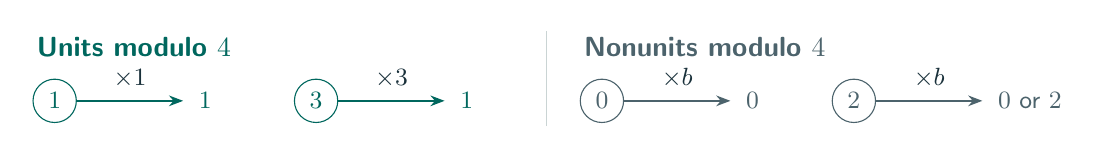
\begin{tikzpicture}[x=1cm,y=1cm,
  residue/.style={circle,minimum size=5.5mm,inner sep=1pt,draw=#1,text=#1},
  product/.style={-{Stealth[length=1.8mm]},line width=.7pt,draw=#1}]
\node[anchor=west,font=\sffamily\bfseries,text=sea] at (0,.69) {Units modulo $4$};
\node[anchor=west,font=\sffamily\bfseries,text=muted] at (6.95,.69) {Nonunits modulo $4$};
\draw[rulegray] (6.6,-.32) -- (6.6,.89);
\foreach \start/\inputclass/\factor/\result/\tone in {
  .35/1/1/{$1$}/sea, 3.67/3/3/{$1$}/sea,
  7.3/0/b/{$0$}/muted, 10.5/2/b/{$0$ or $2$}/muted}{
  \node[residue=\tone] (input) at (\start,0) {$\inputclass$};
  \draw[product=\tone] (input.east) -- ++(1.35,0)
    node[midway,above=1pt,text=ink] {$\times\factor$}
    node[right=2pt,text=\tone] {\result};
}
\end{tikzpicture}
\end{document}
